% Author: Izaak Neutelings (November 2020)
\documentclass[border=3pt,tikz]{standalone}
\usepackage{physics}
\usepackage{tikz}
\usepackage[outline]{contour} % glow around text
\usetikzlibrary{patterns,decorations.pathmorphing}
\usetikzlibrary{decorations.markings}
\usetikzlibrary{bending}
\usetikzlibrary{arrows.meta}
\usetikzlibrary{calc}
\tikzset{>=latex}
\contourlength{1.1pt}

\colorlet{mydarkblue}{blue!40!black}
\colorlet{myblue}{blue!70!black}
\colorlet{myred}{red!65!black}
\colorlet{myorange}{orange!90!black!90}
\colorlet{vcol}{green!45!black}
\colorlet{watercol}{blue!80!cyan!10!white}
\colorlet{darkwatercol}{blue!80!cyan!80!black!30!white}
\colorlet{metalcol}{blue!25!black!30!white}
\tikzstyle{piston}=[blue!50!black,top color=blue!30,bottom color=blue!50,middle color=blue!20,shading angle=0]
\tikzstyle{water}=[draw=mydarkblue,rounded corners=0.1,top color=watercol!90,bottom color=watercol!90!black,middle color=watercol!50,shading angle=20]
\tikzstyle{horizontal water}=[water,top color=watercol!90!black!90,bottom color=watercol!90!black!90,middle color=watercol!80,shading angle=0]
\tikzstyle{metal}=[draw=metalcol!10!black,rounded corners=0.1,top color=metalcol,bottom color=metalcol!80!black,shading angle=10]
\tikzstyle{vvec}=[-{>[flex'=1]},very thick,vcol,line cap=round]
\tikzstyle{force}=[->,myred,very thick,line cap=round]
\tikzstyle{width}=[{Latex[length=4,width=3]}-{Latex[length=4,width=3]}]
\def\tick#1#2{\draw[thick] (#1)++(#2:0.12) --++ (#2-180:0.24)}

\begin{document}


% LAMINAR FLOW around object
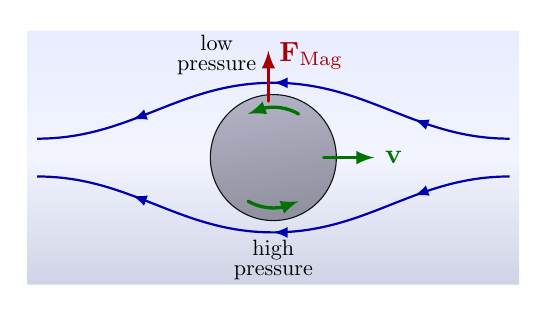
\begin{tikzpicture}
  \def\W{6.0}   % total length
  \def\H{3.1}   % total height
  \def\R{0.8}   % total distance
  
  % WATER
  \draw[water,shading angle=0,draw=none]
    (-0.52*\W,-0.52*\H) rectangle (0.52*\W,0.52*\H);
  \foreach \s in {-1,1}{
    \draw[myblue,thick,postaction={decorate},decoration={markings,
      mark=at position 0.20 with {\arrow{latex}},
      mark=at position 0.50 with {\arrow{latex}},
      mark=at position 0.80 with {\arrow{latex}}}]
      (\W/2,\s*0.3*\R) to[out=180,in=0] (0,{\s*\R+\s*0.2*(\H/2-\R)}) to[out=180,in=0] (-\W/2,\s*0.3*\R);
  }
  
  % OBJECT
  \draw[metal]
    (0,0) circle(\R);
  \draw[vvec] (0.8*\R,0) --++ (0.8*\R,0) node[right] {$\vb{v}$};
  \draw[vvec] (60:0.8*\R) arc(60:120:0.8*\R);
  \draw[vvec] (-120:0.8*\R) arc(-120:-60:0.8*\R);
  \draw[force] (95:0.9*\R) --++ (0,0.8*\R) node[below=2,right] {$\vb{F}_\mathrm{Mag}$};
  \node[below=-3,scale=0.8,align=center] at (-0.12*\W,0.5*\H) {low\\[-1mm]pressure};
  \node[above=-3,scale=0.8,align=center] at (0,-0.5*\H) {high\\[-1mm]pressure};
  
\end{tikzpicture}


\end{document}
